%
%%%%%%%%%%%%%%%%%%%%%%%%%%%%%%%%%%%%%%%%%%%%%%%%%%%%%%%%%%%%%%%%%%%%%%%%%%%
% PDFTEX commands
%%%%%%%%%%%%%%%%%%%%%%%%%%%%%%%%%%%%%%%%%%%%%%%%%%%%%%%%%%%%%%%%%%%%%%%%%%%
%
\pdfoutput=1
\pdfimageresolution=300
\pdfcompresslevel=5
%
%%%%%%%%%%%%%%%%%%%%%%%%%%%%%%%%%%%%%%%%%%%%%%%%%%%%%%%%%%%%%%%%%%%%%%%%%%%
%
\documentclass[twocolumn]{IEEEtran}
%
%%%%%%%%%%%%%%%%%%%%%%%%%%%%%%%%%%%%%%%%%%%%%%%%%%%%%%%%%%%%%%%%%%%%%%%%%%%
%
\usepackage[pdftex]{graphicx}
\usepackage{amsmath}
\usepackage{amsthm}
\usepackage{amsfonts}
\usepackage{amssymb}
\usepackage{cite}
\usepackage{array}
\usepackage{algorithm2e}
\usepackage{url}
\usepackage{xcolor}
\usepackage{xspace}
\usepackage{url}
\usepackage{subfig}
%
%%%%%%%%%%%%%%%%%%%%%%%%%%%%%%%%%%%%%%%%%%%%%%%%%%%%%%%%%%%%%%%%%%%%%%%%%%%%
%
\theoremstyle{definition}
\newtheorem{theorem}{Theorem}
\newtheorem{proposition}{Proposition}
\newtheorem{lemma}{Lemma}
\newtheorem{corollary}{Corollary}
\newtheorem{definition}{Definition}
\newtheorem{example}{Example}
%
% general notation
%
\def\transp{^\intercal}
\newcommand{\refeq}[1]{(\ref{#1})}
\def\opt{\ensuremath{^{*}}}
\providecommand{\argmin}{\mathop{\textup{argmin}}}
\def\gradient{\nabla}
\def\hessian{\nabla^2}
\def\reals{\ensuremath{\mathbb{R}}}
\def\naturals{\ensuremath{\mathbb{N}}}
%
% version control
%
\definecolor{NewTextFG}{rgb}{0.0,0.1,0.8}
\newcommand{\fix}{\marginpar{FIX}}
\newcommand{\pendcite}[1]{{\color{red}[#1]}}
\newcommand{\note}[1]{\colorbox{yellow}{\scriptsize NOTE: #1}} % a la Acrobat
\newcommand{\pending}[1]{{\color{red}\bf PENDING: #1}}
\newcommand{\missing}[1]{{\color{red}\bf MISSING: #1}}
\newcommand{\newtext}[1]{{\color{NewTextFG}{#1}}\xspace}
\newcommand{\patibulo}[1]{{\color{red}{#1}}\xspace}
\newenvironment{textnote}[1]{\colorbox{yellow}{\scriptsize #1$\gg$}}{\colorbox{yellow}{\scriptsize $\ll$}\xspace}
\newcommand{\best}[1]{\textbf{\color{blue}#1}\xspace}
\newcommand{\falta}[1]{{\color{red}FALTA:#1}}
%
%%%%%%%%%%%%%%%%%%%%%%%%%%%%%%%%%%%%%%%%%%%%%%%%%%%%%%%%%%%%%%%%%%%%%%%%%%%%
%
\title{Binary Matrix Factorization via Dictionary Learning}
\author{Ignacio Ram\'{i}rez~\IEEEmembership{Member,~IEEE}\thanks{Departamento de Procesamiento de Se\~{n}ales, Instituto de Ingenier\'{\i}a El\'{e}ctrica, Facultad de Ingenier\'{i}a, Universidad de la Rep\'{u}blica, Uruguay.} }
%
%
%
\begin{document}
%
\maketitle
%
\begin{abstract}
Matrix factorization is a key tool in data analysis; its applications include recommender systems, correlation analysis, signal processing, among others. Binary matrices are a particular case which has received significant attention for over thirty years, especially within the field of data mining. Dictionary learning refers to a family of methods for learning overcomplete basis (also called frames) in order to efficiently encode samples of a given type; this area, now also about twenty years old, was mostly developed within the signal processing field.
In this work we propose two binary matrix factorization methods based on a binary adaptation of the dictionary learning paradigm to binary matrices.
The proposed algorithms focus on speed and scalability; they work with binary factors combined with bit-wise operations and a few auxiliary integer ones. Furthermore, the methods are readily applicable to online binary matrix factorization.
Another important issue in matrix factorization is the choice of rank for the factors; we address this model selection problem with an efficient method based on the Minimum Description Length principle.
Our preliminary results show that the proposed methods are effective at producing interpretable factorizations of various data types of different nature.
\end{abstract}%
\begin{IEEEkeywords}
binary matrix factorization, binary dictionary learning, data mining
\end{IEEEkeywords}
%
\section{introduction}

We consider the problem of approximating a binary matrix $X \in \{0,1\}^{m{\times}n}$ as the product of two other binary matrices $U \in \{0,1\}^{m{\times}p}$ and $V \in \{0,1\}^{n{\times}p}$ plus a third \emph{residual} matrix $E$,
\begin{equation}
X = UV\transp + E.
\label{eq:mf}
\end{equation}
In this work we will consider the $n$ \emph{columns} of $X$ as the data samples to be represented, each of dimension $m$. (Note that this convention, typical in signal processing, is opposite to most works in statistics and computer science, where the \emph{rows} of $X$ are the samples.)
%The problem \refeq{eq:mf} has been addressed using various methods from different fields for over a hundred years. A famous example is Principal Component Analysis (PCA), pioneered by Pearson~\cite{pca}. The PCA method is based on the Singular Value Decomposition (SVD) of a matrix, $X=U{\Sigma}V\transp$ where $U$ and $V$ are matrices of $p=\min\{m,k\}$  orthogonal columns each and $\Sigma$ is a diagonal $p{\times}p$ matrix whose diagonal elements $\sigma_{11} \geq \sigma_{22} \geq \ldots \geq \sigma_{pp} \geq 0$, are the so-called \emph{singular values} of $X$. The PCA method decomposes $X$ by selecting the first $p' \leq p$ columns of $U$, $V$, and upper-left $p'{\times}p'$ submatrix of $\Sigma$ to form an approximation of $X$, $X'=U'\Sigma'(V')\transp$. It can be shown that $X'$ is the rank-$p'$ matrix that best approximates $X$ in Frobenius norm.
%
%Dozens of variants, with different properties, have been developed since PCA was first proposed. Some methods target the robustness of PCA against perturbations in the entries of $X$. This idea was first proposed in~\cite{rpca} and is embodied today by many methods under what is called Robust or Generalized PCA; see~\cite{rpca-paper,rpca-book} for more on the subject. Other methods impose additional restrictions on the factors; a common  one is to enforce $U$ and $V$ in \refeq{eq:mf} to be non-negative, giving rise to the so called Nonnegative Matrix Factorization (NMF) family of methods~\cite{nmf-review}. The restriction of non-negativity is often imposed to improve interpretability  or because the factors are expected to be non-negative by the nature of the problem to be solved (e.g., probabilities). For similar reasons, in different contexts, some matrices cannot be reasonably assumed to be real numbers. If the matrix entries should be integer (or naturals), the usual approach is to treat them as real (or non-negative) numbers anyway and then truncate the result. In other situations, only a relative order between the values can be established. A  more complicated setting is when the entries are just categories or labels (such as Football Teams) for which there is no reasonable relationship  but ``equal'' or ``different''. We call such matrices \emph{categorical}. 

% bmf07 - Zhang, NML proyectado en 0,1. Garantias de recup. bajo hipotesis
% bmf06 -Message Passing for BMF. Además de original, tiene FLOR de review en BMF
% bmf-mdl - ASSO (algoritmo interesante de BMF); MDL casi idéntico al mio
% bmf13 - semi-binario, resuelto con optimización tradicional, pesado, pero
%         con pruebas de solucion exacta en algunos casos.
% falta tiling!!
% bmf-dm - primer paper de Mittienen o algo asi de aplicacion de BMF a data mining
% monson95 - inconseguible, pero citado como 'review de enfoque combinatiorio a BMF
% ASSO: association rule es lo que yo puse como 'correlacion'!
%
The Binary Matrix Factorization (BMF) problem, dating back to at least the 1960's~\cite{bmf-oldest}, has been treated extensively in the last three decades by various research communities, under quite different names. It was first studied as a combinatorial problem as a particular case of the classic \emph{set covering} problem (see~\cite{monson95} and references therein). It then received great attention from the data mining community. The earlier works in this field developed the so called \emph{tiling} or \emph{tile matching/searching} heuristics, where binary matrices are decomposed as Boolean or modulo-2 superpositions of rectangular tiles\cite{proximus,tiling}; it was later formulated as a matrix factorization problem in~\cite{asso}, with several works following that line since then.

A thorough survey of BMF methods is beyond the scope of this paper; we refer the reader to~\cite{bmf-comp} for a more in-depth review. We will however mention some works which are representative of the diversity of formulations and tools that surround the treatment of this problem, as well as the shortcomings that are common to the current state of the art and that motivate the development of the tools that we present in this work.

\subsection{Binary Matrix Factorization}

We begin with the ASSO algorithm proposed in~\cite{asso}. The  method  begins by constructing the so called association matrix $C$, which is a thresholded version of a particular normalization of the correrlation matrix $A{\transp}A$. It then produces a series of increasing rank approximations by adding to $U$ a column taken from $C$ and searching for a corresponding binary row $V_k$ whose outer product with $U_k$ minimizes the number of non-zeros in the current approximation errror $E$. This method can be efficiently implemented with bitwise and integer operations. It is also a popular and simple method with good performance. However, it does not scale well with the number of samples. In particular, for dictionary learning applications where $n \gg m$, the matrix $C$ to be computed can be extremely large, and the overall complexity of each step is $O(kn^2m)$, also very large for values of $n$, something very common in current data science problems.

The work~\cite{bmf07} is one of many examples which use nonlinear optimization over real spaces to solve BMF as a relaxed problem, that is, a Nonnegative Matrix Factorization formulation with values restricted to lie in the range $[0,1]$. The problem solved by~\cite{bmf07} is actually convex and can be solved exactly. Furthermore, if one assumes that $X$ is a noisy observation of a low-rank matrix $\hat{X}$ corrupted by a sparse noise matrix $E$, the solution obtained can be shown to coincide with the sought matrix $\hat{X}$. However, even with modern nonlinear optimization tools, the problem to be solved is computationally very demanding, requiring, as most such methods, repeated computations of the Singular Value Decomposition of a matrix of the same size as $X$.
% bmf13 - semi-binario, resuelto con optimización tradicional, pesado, pero
%         con pruebas de solucion exacta en algunos casos.
% proximus
The work~\cite{bmf13} also poses the BMF problem in terms of a relaxed one, but in this case only one of the factors is assumed binary, while the other is only assumed to be non-negative. Here too, under certain hypothesis regarding an unobserved matrix to be recovered, the result can be shown to coincide with the desired unobserved matrix. As with \cite{bmf07}, the method relies on real nonlinear optimization tools and is thus significantly slower than approximate or heuristic binary-only methods.

The work~\cite{bmf-mp} stands out as an interesting alternative to BMF which formulates the decomposition of $X$ as a Bayesian denoising model with a particular prior on the unobserved \emph{clean} matrix $\hat{X}$ (again, $X=\hat{X}+E$) and uses a Message Passing algorithm to find the maximum a posteriori estimation of $\hat{X}$. Message Passing is a mature technique which in the form presented in this work can be quite computationally demanding. Approximate Message Passing \cite{amp,gamp} techniques have since been developed which may provide significant efficiency gains to the technique proposed in~\cite{bmf06}, but we are currently unaware of any development in this direction.

As an example of a tile-searching method we mention the Proximus method~\cite{proximus}, which approximates the first principal left and right binary components of the binary matrix $X$. The method can be extended to produce a hierarchical representation of the matrix with further rank-$1$ components, although these do not coincide with additional factors in a rank-$k$ factorization. Despite its simplicity, this is a very fast method compared to any of the above methods. Also, as we will see in the next subsection, finding the first principal component of a binary matrix is closely related to a crucial step in one of the main dictionary learning methods. Therefore, we will describe this method in detail later in this document. 

As with any statistical model, the problem of model (order) selection, (in this case, choosing the best rank of the factorization,) is of paramount importance to BMF. Various works~\cite{bmf-mdl,bmf-tiling-mdl,bmf-sel} have addressed this particular problem. In particular,~\cite{bmf-mdl} and~\cite{bmf-tiling-mdl} are based on the Minimum Description Lenght (MDL) principle~\cite{mdl1,mdl2,mdl3}, which forms the basis of our model selection strategy as well. As a side note, the work~\cite{bmf-tiling-mdl} represents a recent example of the tiling approach.

\subsection{Main contribution}

As far as we know, the works in the existing literature on BMF make no particular assumptions on the \emph{shape} of the matrices to be decomposed. As such, despite assigning different roles (such as \emph{factors} for the rows and \emph{loadings} for the columns), most methods treat them symmetrically. Also, most methods deal with the \emph{offline} analysis of 
readily available matrices, which makes them unsuitable to many recent data processing tasks involving \emph{online} adaptation of the models.

We propose a family of methods for BMF which are particularly suited to the treatment of extremely fat (or tall) matrices, which is also suitable to online processing of samples. The proposed methods are, essentially, adaptations to the \emph{dictionary learning} and \emph{sparse coding} techniques which have been developed since the late 1990's~\cite{lewicki99,engan00,aharon06} within the field of signal processing (see see~\cite{dl-review} for a review on both subjects).

In our setting, $X$ is a matrix of $n$ $m$-dimensional column samples which is decomposed as $X=\hat{X}+E=DA+E$, where $D$ is a dictionary of column \emph{atoms}, that is, representative patterns of the data, and $A$ is a \emph{sparse} matrix whose columns dictate the linear combination of columns of $D$ which make up the approximation $\hat{X}$. Another important aspect of dictionary learning methods is that they do not seek low-rank decompositions; the solutions can in fact be \emph{overcomplete}, meaning that the number of columns in $D$ may be larger than $m$, the dimension of the samples to be represented. While dictionary learning can be applied to fixed matrices $X$, efficient online implementations which can adapt both the dictionary and the coefficients as new columns are added to $X$ exist~\cite{online-dl}. We show in Section~\ref{sec:bdl:mod} that the same strategy can be applied to the binary case.

Our methods construct binary dictionaries and binary coefficients matrices using efficient bitwise and a few integer operations. This is particularly relevant to the efficiency and scalability of our method as recent processor architectures incorporate the ability to process large number of bits through SIMD (Single Instruction Multiple Data) instructions. For example, a current off-the-shelf processor can perform a \emph{popcount} instruction (which counts the number of $1$s in a binary array) on a 256-bit register. This allows, for example, to perform the dot product between two binary vectors of dimension $256$ in just two processor instructions. 

The main objective of this paper is to present our proposed methods, study their mathematical properties, and study their empirical performance in terms of convergence, their sensitivity to initial conditions, and their ability to capture structure from different types of data. We thus show and interpret the results obtained with our algorithnms with a small set of easily-interpretable datasets for which the patterns obtained can be visually asserted to correspond to salient features in the data.

The rest of this document is organized as follows: Section~\ref{sec:background:dictionary-learning} provides the notation and background on the methods on which our methods are based. The proposed methods themselves are described in Section~\ref{sec:bdl}.
Section~\ref{sec:model-selection} describes the proposed MDL-based model selection algorithm for searching the best model order $p$. %
We present and discuss our results in Section~\ref{sec:results}, and provide concluding remarks in Section~\ref{sec:conclusion}.

\section{Background}
\label{sec:background}
%
% NOTATION
%
\def\indicator{\mathbf{1}}
\def\bool{\mathrm{bool}}
\def\bprod{\circ}
\def\bsum{\lor}
\def\bigand{\bigwedge}
\def\bigor{\bigvee}
\def\msum{\oplus}
\def\mprod{\otimes}
\def\mod{\mathrm{mod}}
\newcommand{\iter}[1]{^{(#1)}}
\newcommand{\st}{\ensuremath{\quad\mathrm{s.t.}\quad}}
\newcommand{\norm}[1]{\ensuremath{\left\|#1\right\|}}
\newcommand{\support}[1]{\mathrm{supp}(#1)}
\newcommand{\rankf}[1]{\mathrm{rank}(#1)}
\def\rank{\mathrm{rank}}
\newcommand{\fun}[1]{\mathrm{#1}}
\newcommand{\abs}[1]{\ensuremath{\left|#1\right|}}
\newcommand{\setdef}[1]{\ensuremath{\left\{#1\right\}}}
\newcommand{\setspan}{\ensuremath{\mathrm{span}}}
\newcommand{\svec}[1]{_{[#1]}}
\newcommand{\col}[1]{_{#1}}
\newcommand{\row}[1]{^{#1}}
\newcommand{\havg}[1]{\langle\!\langle{#1}\rangle\!\rangle}
%
We will now review the tools on which our implementation is based. We draw both from dictionary learning and data mining methods for this task, thus the section is organized by addressing each set of tools separately. 

We begin by establishing the notation to be used throughout the paper.
Standard operations such as addition or substraction are denoted as usual, $1+1=2$, $1-1=0$, etc. Given two binary values $a$ and $b$, we use $a \land b$ to denote the logical AND (Boolean product) operation between binary operators $a$ and $b$, $a \lor b$ denotes logical OR (Boolean sum),  $a \msum b$ modulo-2 addition (Boolean eXclusive OR), and 1's complement  (Boolean negation) is denoted by $\neg a$. The same notation is used for element-wise operations between vectors and matrices of the same dimension.

Let $x$ and $y$ be two binary vectors and $A$ and $B$ two binary matrices.
We denote the standard  inner and outer vector-vector, matrix-vector and matrix-matrix products as $x{\transp}y$, $xy\transp$, $Ax$ and $AB$.
The Boolean inner product between two vectors, $z = x\transp \bprod y$ is defined as $\bigor x_i \land y_i$. Similarly, the $C_{ij}$ element of the matrix product $C=A \bprod B$ is defined as the Boolean product beetwen the $i$-th row of $A$, $A^i$,  and the $j$-th column of $B$, $B_j$. We define the modulo-2 inner product of $x$ and $y$ as $x \mprod y = (x+y)\;\mod \;2$. Finally, similarly to the boolean case the $C_{ij}$ element of the modulo-2 product between two matrices, $C=A \mprod B$ is given by $A^i \mprod B_j$. 

The number of elements or size of a set $J$ is denoted by $|J|$. 
For a vector $x$, its Hamming weight $h(x)$ is defined as the number of non-zero elements in $x$, that is $h(x)=|\{i: x_i \neq 0\}|$. In dictionary learning and sparse coding jargon, the Hamming weight is referred to as the $\ell_0$ pseudo-norm, $\|x\|_0=h(x)$. Note that, for binary vectors, $h(x)=\|x\|_0=\|x\|_1=\norm{x}_2^2$. The function $\indicator(\cdot)$ is defined so that $\indicator(cond)=1$ if $cond$ is true, and $0$ otherwise. 
Finally, we define the \emph{Hamming average} of a binary vector of length $m$  as $\havg{x} = \indicator(h(x) \geq m/2)$, that is, $1$ if the at least half of the elements of $x$ are nonzero. Likewise, for matrices, we define $h(A)$ as the number of nonzero elements in $A$.

\subsection{Dictionary Learning and sparsity}
\label{sec:background:dictionary-learning}
%
The aim of \emph{Dictionary Learning} methods is to obtain efficient representations of specific types of signals in terms of basis or \emph{frames} which are adapted to the particularities of the signal type at hand (see~\cite{dl-review} for a review). This is in contrast to the traditional approach where fixed transforms such as the Discrete Fourier Transform (DFT) or any of the wide family of Discrete Wavelet Transforms (DWT) are used to compactly represent the salient features of signals such as audio tracks or natural images. In this setting, the columns of $X$ are data samples, for example short audio segments or pixel values from patches of natural images. The dimension $m$ of the data samples is usually much smaller than the number of samples $n$. In the more general context of matrix factorizations, we say that these are extremely \emph{fat matrices}; this is an important aspect to consider in MF algorithms, as we will see later.
For sufficiently large $n$, we can tailor a \emph{dictionary} $D \in \reals^{m{\times}p}$ such that each sample in $X$ can be compactly represented in terms of a few columns of $D$; by compact we mean that we can represent $X=DA+E$ with $\|E_i\| \ll \|X_i\|$ and $\|A_i\|_0 \ll p$.

As we can see from the previous discussion, contrary to the more general MF approach where the factors $U$ and $V$ have similar roles, those of $D$ and $A$ are quite different. The columns of the matrix $D$ are called ``atoms'' and are supposed to embody typical patterns observed throughout the columns of $X$, while the columns of $A$ specify the linear combination of columns of $D$ that better approximates the corresponding columns of $X$.

A typical approach to the generally non-convex Dictionary Learning problem is to obtain a local solution by alternate minimization in $D$ and $A$,
%
\begin{eqnarray}
A\iter{k+1} =& \arg\min_{A} \{ f(D\iter{k}-A) + g(A) \} \\
D\iter{k+1} =& \arg\min_{D} \{ f(D-A\iter{k+1}) + g(A\iter{k+1}) \},
\label{eq:dl}
\end{eqnarray}
%
where $f(\cdot)$ and $g(\cdot)$ are \emph{fitting} and \emph{regularization} functions respectively. We now describe  the two  methods on which our methods are based.

\subsubsection{Method of Optimal Directions (MOD)} 
\label{sec:mod}
For the case $f(D,A)=\|DA-X\|_2^2$ and $g(A)=\sum_{i}\|A_i\|_1$ the \emph{Method of Directions} (MOD)~\cite{mod}, is given by
\begin{eqnarray}
A_j\iter{k+1}\!\! &=&\!\! \arg\min_{a \in \reals^p} \{ \|x_j - D\iter{k}a \|_2^2 + \|a\|_1, \} \\
D_r\iter{k+1}\!\! &=&\!\! U_r/\min\{1,\|U_r\|_2\},\nonumber\\
\!\!&&U=\!\!X(A\iter{k+1})\transp\left(A\iter{k+1}({A}\iter{k+1})\transp\right)^{-1},\,
\label{eq:mod}
\end{eqnarray}
where $A_j$ and $D_r$ are the $j$-th and $r$-th columns of $A$ and $D$ respectively. The first step corresponds to an $\ell_1$-regularized least squares regression problem on each column of $A$, also known as LASSO~\cite{lasso}, a non-differentiable convex problem whose solution has been extensively studied in recent years, with several efficient algorithms designed especifically for the task (see e.g.~\cite{fista}).
In the second step, each atom $D_r$ of the dictionary corresponds to a normalized down version of the least squares solution $u_r$. Here too, (although not ``officially'' part of the algorithm,) it is customary  to apply some sort of regularization so that the Hessian matrix $AA\transp$ is invertible and well conditioned.

The MOD algorithm is well suited for online dictionary adaptation, as both  $A{A}\transp$ and $XA\transp$ can be efficiently updated when new columns are added to $X$. Furthermore, if new samples arrive one at a time, the inverse of the Hessian matrix $({A}A\transp)^{-1}$ can be efficiently updated via the matrix inversion lemma~\cite{matrix-inv-lemma}. Moreover, as shown in~\cite{online-dl}, excellent results are still obtained by this method if the full Hessian is approximated by its diagonal (in which case its inverse is trivial to compute and update).

\subsubsection{The K-SVD algorithm} 
\label{sec:ksvd}

In this algorithm, proposed in~\cite{aharon06}, $f(E)=\norm{E}_2$ and $g(\cdot)=h(A)$. The columns of $A$ are computed using a greedy method known as OMP (Orthogonal Matching Pursuit)~\cite{omp}, which   under certain conditions can be shown to provide the actual solution to the corresponding $\ell_0$-penalized least squares problem (see~\cite{tropp07}). A simpler variant of this step uses the (non-orthogonal) Matching Pursuit (MP)~\cite{mp}, which is described next in Algorithm~\ref{alg:mp}, 
%
\begin{algorithm}[ht] 
\caption{\label{alg:mp}Matching Pursuit}
\KwData{vector to encode $x$, dictionary $D$, maximum residual norm $\epsilon$, maximum coefficients weight $k$}
\KwResult{Coefficients vector $a$}
Set iteration $t \leftarrow 0$, residual $r\iter{0} \leftarrow x$, initial coefficients $a\iter{0} \leftarrow 0$\;
Set $g\iter{0} \leftarrow D\transp{r\iter{0}}$, $G \leftarrow D\transp{D}$ \;
\While{$\norm{r\iter{t}} \geq \epsilon$ and $h(a) < k$}{
  $i = \arg\max \left\{g\iter{t} \right\} $ \;
  ${\Delta} \leftarrow D_i\transp r\iter{t}$ \;
  $a_i\iter{t+1} \leftarrow a_i\iter{t} + \Delta$ \;
  $r\iter{t+1} \leftarrow r\iter{t} - {\Delta}D_i $\; 
  $g\iter{t+1} \leftarrow g\iter{t} - {\Delta}G_i $\tcc*{(a)} 
  $t \leftarrow t+1 $ \;
}
\Return $a \leftarrow a\iter{t}$ \;
\end{algorithm}
%
What MP does at each iteration is to project the residual onto the atom that is most correlated to it, and then remove the projection from the residual. For this to work well, the atoms must be normalized to have $\ell_2$ norm 1.
The vector $g$ keeps track of the correlation between the residual $r$ and the dictionary $D$.  Its update $(a)$ is derived as follows: 
\begin{eqnarray}
g\iter{t+1}
 &=& D\transp{r\iter{t+1}}=D\transp(r\iter{t}-{\Delta}D_i)\nonumber\\
 &=& g\iter{t}-{\Delta}D\transp{D_i} =g\iter{t}-{\Delta}G_i.
\label{eq:corr-up}
\end{eqnarray}
Note that, by means of \refeq{eq:corr-up}, updating $g$ requires only $2p$ floating point operations, whereas the na\"{i}ve update requires $mp$ operations.  As we will see later, this same trick, with a few modifications, will also be useful in the binary case.

The dictionary update of K-SVD performs a simultaneous update of each atom $D_r$ and the row of $A$ associated to it. This update is described in Algorithm~\ref{alg:ksvd}. 
%
\begin{algorithm}
\KwData{Current model $D\iter{t}$, $A\iter{t}$ and $E\iter{t}=X-D\iter{t}A\iter{t}$}
\KwResult{Dictionary and coefficients for next iteration $D\iter{t+1}$,$A\iter{t+1}$}
\For{$r=1,\ldots,p$}{
  $R \leftarrow X - D\iter{t}A\iter{t} + D\iter{t}_r(A\iter{t})^r$ \;
  $U{\Sigma}V\transp \leftarrow \mathrm{SVD}(R)$ \;
  $D_r \leftarrow U_1$ \;
  \tcc{\small $A^r_{nz}$ are the non-zero entries of $A^r$}  
  $A^r_{nz} \leftarrow V_1$ \;
}
\Return $(D,A,E) \leftarrow (D\iter{t},A\iter{t},E\iter{t})$ \;
\caption{\label{alg:ksvd}K-SVD Dictionary update.}
\end{algorithm}

The dictionary update described in Algorithm~\ref{alg:ksvd} is significantly more costly than that of MOD, (even if only $U_1,\Sigma_{11}$ and $V_1$ are computed) but usually requires less iterations to converge to a good result. However, unlike MOD, K-SVD is not well suited for online adaptation as it involves the re-computation of the (partial) SVD each time a new sample is added.


\section{Binary Dictionary Learning}
\label{sec:bdl}

Given a particular model order (determined by the dictionary size) $p$, our proposed methods consist of a traditional alternate descent dictionary learning approach much like MOD and K-SVD. On top of it, we use the Minimum Description Length (MDL) criterion for evaluating the parsimony of the best learned model of size $p$, together with a top-level MDL-based model selection algorithm for choosing the best order $p$ within a range $0 \leq  p_{\min} \leq p \leq  p_{\max}$. We leave the description of the top-level model selection algorithms to Section~\ref{sec:model-selection}.

Both BMF algorithms share a common coefficients update step, the Binary Matching Pursuit (BMP) algorithm, and  two choices for the dictionary update step: MOB (a binarized version of MOD) and K-PROX (combining ideas of K-SVD and Proximus)  We now provide details on each of these new algorithms.

\subsection{Coefficients update via Binary Matching Pursuit (BMP)}
\label{sec:bdl:bmp}

In essence, BMP is a binarized version of the Matching Pursuit Algorithm~\ref{alg:mp}. For a given sample $x$, we begin ($t=0$) with an initial coefficients vector $a\iter{0}=a_0$, a residual $r\iter{0}_j=x \oplus D \mprod a\iter{0}$ and an initial vector $g\iter{0}=D\transp x$ which keeps track of the \emph{Euclidean} (traditional)  correlation between the columns of $D$ and $r\iter{t}$. Then, at each iteration $t$ we \emph{toggle} the coefficient $a_j(k)$ corresponding to the atom that is most correlated to $r\iter{t}$, $D_{k}$, and $D_k$ is accordingly modulo-2 added to $r\iter{t}$. The pseudocode is given in Algorithm~\ref{alg:bmp}. 
%
\begin{algorithm}[ht]
\KwData{sample to encode $x$, dictionary $D$, initial coeficients $a_0$, maximum steps $t_{\max}$, maximum residual weight $w_{\max}$, residual exponent $\beta$}
\KwResult{Optimum coefficients for $x$, $a$}
Set iteration $t=0$, coefficients $a\iter{0}=a_0$ ,residual $r\iter{0}=x \oplus D{\mprod}a\iter{0}$\;
Set modulo-2 Gramm matrix $G = D\transp \mprod D$\tcc*{(a)}
Set residual correlation $g\iter{0}=D\transp{r\iter{0}}$\tcc*{(b)}
\While{$h(r\iter{t}) \geq w_{\max}$ \textbf{and} $t < t_{\max}$ }{
  $k \leftarrow \arg \max_l \{\;|g\iter{t}_l|\;/\;\|D_l\|_2^\beta\;\} $ \tcc*{(c)}
  \If{$g\iter{t}_{k} = 0$} { 
  	  \Return $a \leftarrow a\iter{t}$ \; 
  }  
  $r\iter{t+1} \leftarrow r\iter{t} \oplus  D_{k} $\; 
  \If { $h(r\iter{t+1}) \geq h(r\iter{t})$\tcc*{(d)} } 
  {
	  \Return $a \leftarrow a\iter{t}$ \;
  }
  \eIf {$a\iter{t+1}_{k} = 1$} {
    $a\iter{t+1}_{k} \leftarrow 0$ \;
    $g\iter{t+1} \leftarrow g\iter{t} - G_{k}$\tcc*{(e)}
    } {
    $a\iter{t+1}_{k} = 1$ \; 
    $g\iter{t+1} \leftarrow g\iter{t} + G_{k}$ \tcc*{(e)}
    }
} 
\Return $a \leftarrow a\iter{t}$ \;
\caption{\label{alg:bmp} Binary Matching Pursuit.}
\end{algorithm}

Some steps of the algorithm, marked as $(a)$, $(b)$, $(c)$, $(d)$ and $(e)$ (appearing twice) are not obvious from the overall description of the algorithm and need to be clarified. 

In $(a)$, the \emph{modulo-2 Gramm matrix} of $D$ is computed. This matrix is used in an analogous way in Algorithm~\ref{alg:mp} for the fast update of the correlations vector $g$ as described in \refeq{eq:corr-up}. Despite the fact that we are working with binary vectors with binary operations, the euclidean correlation $(b)$ between the dictionary and the residual  is still a good proxy for choosing an atom that will serve to reduce the weight of the residual. Note however that this will work correctly if the atoms are normalized, which they are not. This is why 
the maximum in $(c)$ is taken with respect to the ratio $g\iter{t}_l / \|D_l\|_2^\beta$, which corresponds to the empirical Pearson correlation for $\beta=1$ (the inclusion of $\|r\iter{t}\|_2$ in the denominator is irrelevant for minimization purposes). In our experiments we use $\beta=2$, which corresponds to the so called \emph{association accuracy} in data mining~\cite{association-accuracy}. 

The step marked with $(d)$ adds monotonicity to the method: if the weight of the residual increases (which might happen), the update is rolled back and the algorithm finishes.

Finally, and most interestingly, despite the correlation vector $g$ being initially computed using the \emph{standard} matrix-vector product, it can be updated using exactly the same form as \refeq{eq:corr-up}, only that the Gramm matrix $G$ is actually computed using the modulo-2; The first $(e)$ corresponds to the case when $\Delta=1$, that is, when $a_k$ is switched from $0$ to $1$. The second $(e)$ corresponds to $\Delta=-1$, when $a_k$ is switched off. (This curious result is easily verified by writing down the corresponding arithmetic.) 

%
%\subsection{Coefficients update/Binary Weight Pursuit (BWP)}
%
%\begin{algorithm}[ht]
%\KwData{sample to encode $x$, dictionary $D$, initial coeficients $a$, maximum steps $t_{\max}$, maximum residual weight $w_{\max}$}
%\KwResult{Optimum coefficients for $x$, $a$}
%Set iteration $t=0$, residual $r\iter{0}=x$, coefficients $a\iter{0}=a$\;
%Set residual correlation $g\iter{0}=D\transp{r\iter{0}}$ \;
%\While{$h(r\iter{k}) \geq w_{\max}$ \textbf{and} $t < t_{\max}$ }{
%  $h_{\min} \leftarrow \min h(D_i \oplus r\iter{k}) $ \;
%  \If{$h_{\min} > h(r\iter{k})$} { break }  
%  $i \leftarrow \arg\min h(D_i,r\iter{k}) $ \;
%  $a_i  \leftarrow  {a}_i  \oplus 1 $ \;
%  $r\iter{k+1} \leftarrow r\iter{k} \oplus  D_i $\; 
%  
%}
%\label{alg:bmp}
%\end{algorithm}
\subsection{MOB: Method Of Binary Directions}
\label{sec:bdl:mod}
 
Here we want to update each atom so that the Hamming weight of the total residual matrix $E = X \oplus D \mprod A$ is minimum (we recall that minus and plus are the same thing in modulo-2 arithmetic). Say we want to update the $r$-th atom at iteration $k$. Clearly, the affected columns will only be those for which the  coefficients in $A$  corresponding to that atom are non-zero, that is $\{j : A_{rj} \neq 0 \}$; let us call this set $J_r$ and $n_r$ its size. What we want is the update $\Delta$ that, when added to $D_r$, minimizes the weight of the residual $E$ in those colums affected by $D_r$,
 \begin{eqnarray}
 \Delta  =& \arg\min_d \sum_{j \in J_r}  h(E\iter{k}_j \oplus d) \\
 =& \arg\min_d \sum_{j \in J_r} (\sum_i E\iter{k}_{ij} + n_r d_i).
\label{eq:mob1}
 \end{eqnarray}

According to~\refeq{eq:mob1}, the optimization of $\Delta$ is trivially separable as,
 \begin{eqnarray}
 \Delta_i  =& \arg\min_{u \in \{0,1\}} \sum_j E_{ij}\iter{k} \oplus u\\
 =& \arg\min_{u \in \{0,1\}} \sum_{j\in J_r} E_{ij} + n_r u.
\label{eq:mob2}
 \end{eqnarray}
In other words, the $i$-th element of $D_r$ should be $0$ if most of the elements in the rows of $E$ affected by it are $0$, and $1$ otherwise. 
This is clearly an optimum solution (note that there could be many optima  when $n_r$ is even, in which case we simply choose one value; in our case we use $0$).

We now observe that, at any given step of the algorithm, the $r$-th diagonal element of the Hessian matrix $(AA\transp)_{rr}=n_r=h(A^r)$, and that $\sum_{j\in J_r} E_{ij}\iter{k}=E(A^r)\transp(1/n_r)$. Therefore, the update \refeq{eq:mob2} can be seen as a binarized version of the dictionary update proposed in~\cite{online-dl}, that is, 
$$D_r = \indicator\left(\frac{E(A^r)\transp}{h(A^r)} \geq \frac{1}{2}\right).$$
From the above observations, it follows that MOB can also be used for fast online dictionary adaptation, as both $n_r$ and $E(A^r)$ can be easily updated as new samples arrive. (Our implementation of this feature is still work in progress.)

\subsection{K-PROX: Dictionary Update via Proximus}
\label{sec:bdl:k-prox}

In this case, following the K-SVD concept, we want to obtain the best rank-one approximation to the residual $E$ obtained after removing the contribution of $D_r$. Let $J_r = \{j: A_{rj} \neq 0 \}$ and $E_{J_r}$, $X_{J_r}$ and $A_{J_r}$ the submatrices formed by the columns of $X$ and $A$ indexed by $J_r$ and $R_{J_r}=D{\mprod}A_{J_r} \oplus E_{J_r}$. We then have the following update:
\begin{equation}
(D_r\iter{k+1},A_{J_r}\iter{k+1}) = \arg\min_{u,v} h\left( R_{J_r}\iter{k} \oplus uv\transp \right).
\label{eq:bsvd1}
\end{equation}
As the name K-PROX implies, we seek an approximation to the NP-hard problem \refeq{eq:bsvd1} using the Proximus algorithm~\cite{proximus}, which we summarize in Algorithm~\ref{alg:proximus},
%
\begin{algorithm} 
\caption{\label{alg:proximus} Proximus}
\KwData{matrix $X \in \{0,1\}^{m{\times}n}$, $u\iter{0} \in \{0,1\}^m$, $v\iter{0} \in \{0,1\}^n$ }
\KwResult{Vectors $u$, $v$ so that $X \approx uv\transp$}
Set iteration $k=0$\;
\Repeat {$u\iter{k}(v\iter{k})\transp = u\iter{k-1}(v\iter{k-1})\transp$} {
  $u\iter{k+1}_i\!\! \leftarrow \indicator \left( A^i v\iter{k} > \|v\iter{k}\|_0/2 \right),\;i=1,\ldots,m$ \;
  $v\iter{k+1}_j\!\! \leftarrow \indicator\left(A_j\transp{u\iter{k+1}}\!>\!\|u\iter{k+1}\|_0/2 \right),j=1,\ldots,n$ \;
  $k \leftarrow k+1 $ \;
}
\end{algorithm}
%
Interestingly, Algorithm~\ref{alg:proximus} provides a local optimum to the rank-one approximation that we seek. This is stated in Proposition~1 below.
\begin{proposition}
The output $(u,v)$ of the Proximus Algorithm~\ref{alg:proximus} is a local optimum of the problem $\min \|X - uv\transp\|_0$. 
\end{proposition}
\begin{proof}
 Given $v\iter{k}$, it is easy to check that the update $u\iter{k+1}$ in Algorithm~\ref{alg:proximus} is the value of $u$ that \emph{globally} minimizes $\|X \oplus uv\iter{k+1} \|$ (if $ s\iter{k}_i = w\iter{k}/2$, both $0$ and $1$ are equally optima; in such case, we default to $0$). The same happens with the update $v\iter{k+1}$ given $u\iter{k+1}$. Therefore, $h(E\iter{k})=h(X \oplus u\iter{k}(v\iter{k})\transp)$ cannot increase with $k$. As $h(E\iter{k}) \geq 0$ is bounded, non-increasing, and the iterates can take on a finite number of values, the sequence $h(E\iter{k})$ must converge  after a finite number of steps. Let $(u,v)$ be the arguments at which the stopping condition is satisfied. By definition of the algorithm, no change in $u$ or $v$ decreases the objective. This guarantees that $(u,v)$ is a local minimum in a Hamming ball of radius at least $1$.\footnote{notice that we cannot guarantee that a simultaneous change in a single coordinate of $u$ and a single coordinate of $v$ will not decreasae the cost function!.} 
\end{proof}

%\subsection{Initialization}
%\label{sec:proximus:init}
%
%Initialization is always a serious issue in non-convex problems, particularly in dictionary learning methods. The binary case is no exception. The authors of Proximus propose a number of initialization methods, namely: 
%
%\paragraph{partition} The authors propose to choose one \emph{separator} column (they do not specify how) and then use that column, along with the Hamming centroid of the rows for which the corresponding value in the separator column is $1$.
%\paragraph{greedy graph growing} Let $P$ be a subset of rows whose only initial element is a randomly select row. Then, recursively add all rows which share a non-zero location with \emph{any} row currently in $P$ until no additional rows can be added. The initial pattern vector $v$ is the Hamming centroid of the rows in $P$.
%\paragraph{neighbor} Similar to greedy graph growing, but less greedy, this one chooses a pivot row at random and initializes the pattern vector to the Hamming centroid of all the rows that share at least one non-zero location with the pivot row.
%
%The above initialization heuristics are not claimed to be good in any sense; they just embody some principles and practices usually seen in Data Mining applications. A careful analysis of each method is beyond this paper. However, it is important to shed some intuition as to how these methods would perform in the $n \gg m$ setting found in dictionary learning problems.
%Also, it is important to consider that these initialization methods are designed for a rank-one decomposition and might be unsuitable or require modifications to work for rank-k factorizations. We will discuss these issues in the context of the proposed methods, which are described in the next section.
%

\subsection{Initialization}
\label{sec:bdl:init}

Initialization is of paramount importance to the success of any non-convex matrix factorization method. At the same time, there is no provably optimum way of doing so, otherwise we would be contravening the NP-hard nature of the factorization problem itself. We are left with heuristics based on intuition and prior information, if any. Ultimately, \emph{initialization is an art}. Below we describe the three methods we have tested with our algorithms, two of which are vaguely inspired by the ones proposed in Proximus (which are defined only for rank-$1$ factorizations.) In any case, these are not to be taken as particularly good methods; they are examples which in some cases, as we will see, can work well. 

\paragraph{(Pseudo) Partition}: This method works for dictionaries of size $p \leq m$. Let $I=\{i_1,i_2,\ldots,i_p\}$ be the indexes of the $p$ rows of $X$ which have the largest weight, that is, $h(X_i) \geq h(X_{i'}),\forall\,i\in{I},\,i' \notin{I}$. Then the $k$-th atom is initialized as the Hamming average of all the \emph{columns} of $X$ which have a $1$ in their $i_k$-th row. If we define $J_k=\{j:1 \leq j \leq n, X_{i_kj}=1 \}$, then $$D_k = \frac{1}{|J_k|}\sum_{j \in J_k} X_j.$$ 
The idea behid this initialization is to ensure that the initial atoms are correlated with those dimensions which are more commonly active in the dataset; this is particularly useful in very sparse matrices, but for the same reason can fail for dense matrices as all the atoms may end up being mostly $1$ and very similar among themselves.
 
\paragraph{Neighbor}: Here we draw $p$ samples at random from $X$, then each atom $D_k$ is initialized as the Hamming average of all samples in $X$ which have non-zero correlation with $X$. This is essentially a rank-$k$ extension of the method described in \cite{proximus} under the same name. It is however not a good method for dense, fat matrices (see Figure~\ref{fig:init-mnist} on page~\pageref{fig:init-mnist}), especially if some row of $E$ is largely composed of $1$s, in which case all or most atoms may end up being identical, dense patterns.

\paragraph{Random} This is a fallback, universal alternative for initializing a dictionary when almost no prior information can be exploited to devise a better alternative. The samples are initialized using pseudo-random Bernoulli samples of probability $\theta$, a parameter which can be chosen to reflect, for example, the density of $1$s in the dataset.  The value by default is $1/2$, which is a good idea even for very sparse matrices, as $\theta \ll 1$ combined with a large dimension $m$ may result in atoms which are orthogonal to most or even all data samples if the data is sparse.


%\subsection{Learning variants}
%
%I implemented several variants of the above algorithms, most of them just change the order in which some updates are made, or switch the roles of dictionary and coefficients alternatively, so that the method can be used on a broader class of data.
% 
%
%\begin{enumerate}
%\item Traditional: traditional alternate descent until local convergence
%\item Role-switching I: at each iteration, the role of A and D are switched
%\item Role-switched learning II: after local convergence (the same as in the first case), the role of A and D are switched and the traditional model is applied again
%\item Role switched learning III: like type I but only the dictionary update step is applied (for use with Proximus)
%\end{enumerate}

\section{Model selection}
\label{sec:model-selection}

A crucial problem in BMF is how to choose the appropriate rank $p$ of the decomposition. In dictionary learning, this translates into the number $p$ of atoms of the dictionary $D$. This is a particular case of what is generally known as the \emph{model selection} problem. 

Beyond theoretical results and simulations, when confronted with real data, 
the true underlying model governing the generation of data is rarely available. In such situations, models can only be assumed to be tools for understanding the data at hand, and the best choice is dictated by how much regularity or structure each candidate model is capable to grasp from that data. In particular, the complexity of a model is limited by the amount of data available to estimate the different parameters of the model. An overly complex model will tend to \emph{overfit} the data, whereas an overly simple one will miss important details. The problem of model selection is that of finding the best model for a given data set. Typically this is done by seeking a balance between the \emph{goodness of fit} of a model, usually expressed in terms of the likelihood of the data given the model, and a measure of the \emph{model complexity}; two very popular examples in this category are the Bayesian Information Criterion (BIC)~\cite{bic}, the Akaike's Information Criterion~\cite{aic}. 

The Minimum Description Length principle (MDL)~\cite{mdl1,mdl2,mdl3} translates the model selection problem as one of data compression, where both the data and the model have to be (hypothetically) transmitted and perfectly recovered using some encoding mechanism. The tension between complexity is then resolved by how many bits are required to describe the data in terms of the model (stochastic complexity) and how many bits are required to describe the model itself (model complexity). The original version of MDL~\cite{mdl1} made this division explicit, and is asymptotically equivalent to BIC. However, the modern version of MDL~\cite{mdl2,mdl3} uses the more recent information-theoretic \emph{universal coding theory} to make the aforementioned balance implicit by producing an optimum, joint description of both the model and the data which is furthermore independent of arbitrary choices of, for example, the way the model is parameterized. These advantages make MDL an appealing method for model selection. However, contrary to BIC and AIC, MDL is more difficult to implement, in particular in its modern version. 

In this section we describe a particular implementation of the MDL criterion for BMF models. This consists of two pieces. The first one is how to compute the hypotethical optimum codelength of our matrix $X$ given  a candidate factorization $(E,A,D)$. This has to be done with reasonable accuracy and efficiently. The second one is how to search over the possible models; simply trying out every possible model is clearly out of question.

\subsection{Codelength computation}

The universal compression of binary sources has been extensively studied in the literature. Moreover, we do not need to perform a real encoding; we need only to compute the codelength. One particularly simple method, for which the codelength is easy to compute, is \emph{enumerative coding}~\cite{enum}. Given a binary string $x$ of length $n$ ahd its hamming weight $r=h(x)$, its enumerative code is composed of two parts. The first one describes $r$ with $\lceil\log_2(n)\rceil$ bits, and the second one describes the index of $x$ in the lexicographically ordered list of all strings of length $n$ with the same weight $r$, which requires $\lceil\log_2{r \choose n}\rceil$ bits. The total codelength is then $$L(x) = \lceil\log_2(n)\rceil + \lceil\log_2{r \choose n}\rceil.$$ (Note that $\log{r \choose n}$ can be accurately approximated by using Stirling's formula, a function which is readily available in most scientific computation libraries.)
As we expect the different columns of $D$ to represent particular patterns in the data, and the corresponding rows of $A$ their appearance in $X$, it makes sense to consider different codes for each column and row of $D$ and $A$ respectively. As of $E$, the usual assumption is to consider it as \emph{noise}. While this may not always be the case (remaining structure may still exist in $E$ after the decomposition), it is a safe and general assumption. Thus, we encode the whole matrix $E$ as one single binary string of length $m{\times}n$. The total codelength for our model is then givem by
\begin{equation}
L(X) = L(E) + \sum_k [ L(D_k) + L(A^k) ] 
\label{eq:codelength}
\end{equation} 
The codelength function~\refeq{eq:codelength} encoding scheme is among the ones proposed in~\cite{bmf-mdl}.

\subsection{Model selection}

Given the codelength function $L(X)$, we now need to solve: a) the search for the best model given $p$ and b) the best value of $p$. The first problem is what most of this paper is about, that is, to learn the dictionary and coefficients $A$, and is described in Section~\ref{sec:bdl}. In order to choose the best order $p$ of the model we apply a \emph{forward selection} strategy. We begin with an initial dictionary size $K=K_{\min}$, adapt it to the data, add one or a few more atoms to $D$, and re-adapt both $D$ and $A$. The previous step is repeated until no further improvement is obtained, that is, until the overall codelength $L(X)$ does not decrease by adding new atoms to the dictionary.

\section{Results and discussion}
\label{sec:results}

\begin{figure*}[p]
\centering%
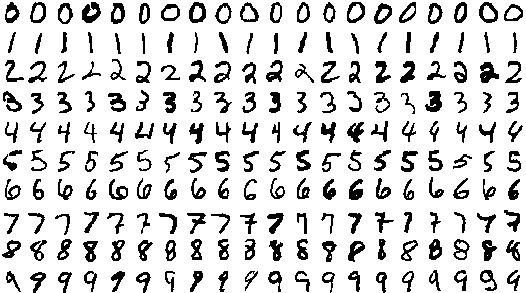
\includegraphics[height=1.6in]{fig/mnist_bin.png} %
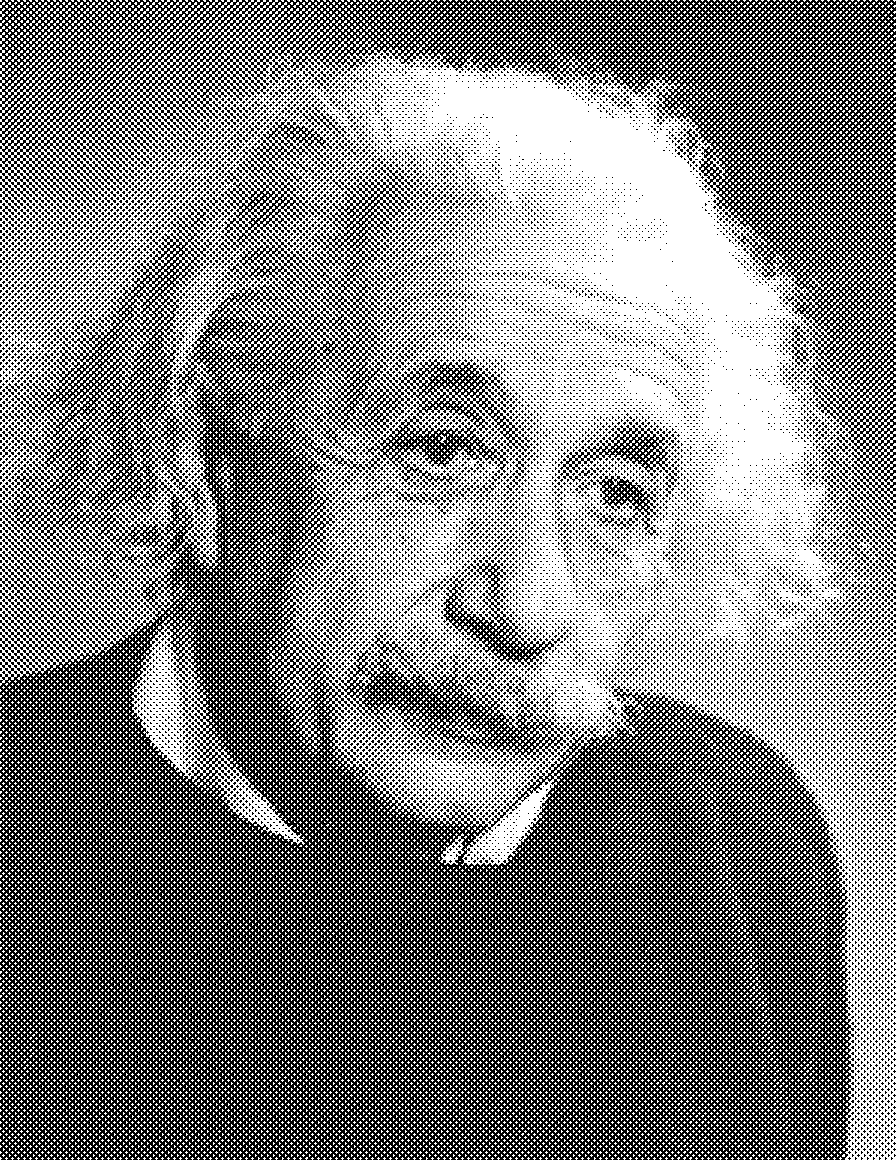
\includegraphics[height=1.6in]{fig/einstein.png} %
%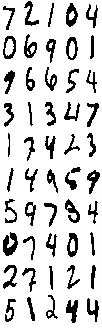
\includegraphics[height=1.8in]{fig/usps_b.png} %
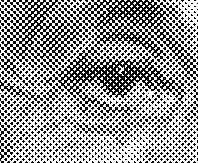
\includegraphics[height=1.6in]{fig/einstein_zoom3.png}
\caption{\label{fig:datasets} Left to right: MNIST dataset, Einstein image, USPS dataset,  detail of Einstein's left eye.}
\end{figure*}
%
The following results were obtained with our current implementation, which can be download fromt \url{http://iie.fing.edu.uy/~nacho/bdl/}, and which includes scripts that reproduce all the results shown in this section and many more. The results shown are for binarized version the handwritten digits dataset MNIST~\cite{mnist} and for the halftone binary image of Einstein. Both datasets have easily visually interpretable patterns, which helps in assessing the quality of the obtained models. Figure~\ref{fig:datasets} shows a few samples from MNIST, the Einstein image, and a detail of his eye which shows the halftoning pattern. The MNIST dataset consists of $10000$ $16{\times}16$ grayscale images of hand written digits. For Einstein, the samples consist of the $4088$ non-overlapping blocks of size $16{\times}16$ that the image can be decomposed into.

\subsection{Models}

\begin{figure*}[tp]
\centering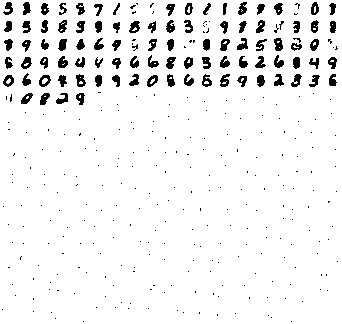
\includegraphics[height=2.2in]{fig/mnist_mob_dict.png}\hspace{2ex}%
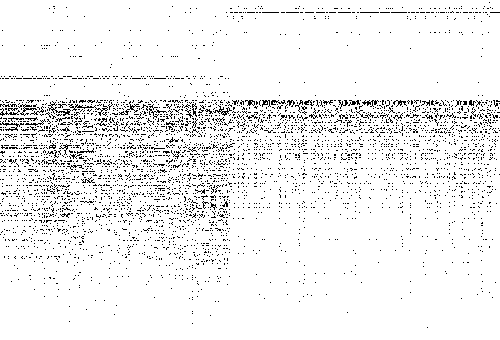
\includegraphics[height=2.2in]{fig/mnist_mob_coef_crop.png}%\\
%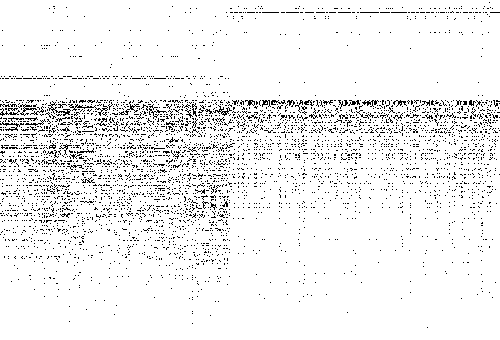
\includegraphics[width=\columnwidth]{fig/mnist_mob_coef_crop.png}
\caption{\label{fig:mnist-mob} Sample model obtained for the MNIST dataset using the MOB method. The best order here is $p=340$, which is greater than the data dimension $m=256$. The residual $E$ negligible, with only $h(E)=2630$ nonzero elements in a matrix of $2.560.000$ entries. On the left we show the dictionary, comprised mostly of digits of various shapes and then a large number of small details. The picture to the left corresponds to the rows of $A$ corresponding to samples $750$ to $1250$, spanning the last $250$ $0$s and the first 250 $1$s in the dataset; note the different activation patterns between the two.}
\end{figure*}
%
\begin{figure*}[tp]
\centering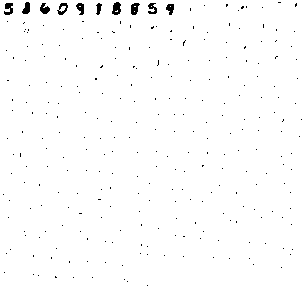
\includegraphics[height=2.0in]{fig/mnist_kprox_dict.png}\hspace{2ex}% 
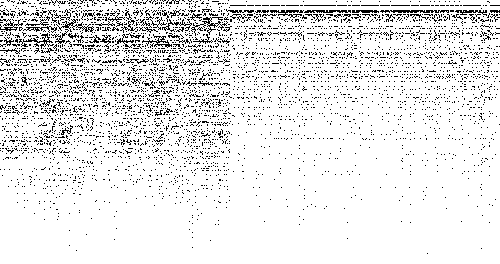
\includegraphics[height=2.0in]{fig/mnist_kprox_coef_crop.png}%\\
%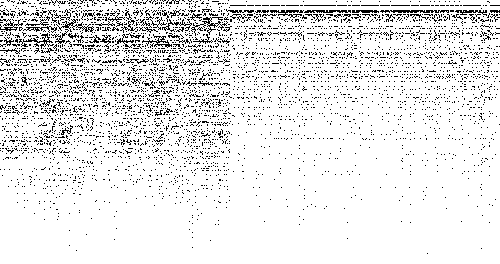
\includegraphics[width=\columnwidth]{fig/mnist_kprox_coef_crop.png}
\caption{\label{fig:mnist-kprox} Model obtained for the MNIST dataset using K-PROX. A similar situation occurs in this case, with $p=264$ and a dictionary which consists of $10$ digits closely resembling digits and then a number of atoms whose function appears to be the correction of the crude approximations obtained after using the first $10$ atoms. Here again the final weight of $E$ is just $h(E)=2615$, but  the coefficients matrix (of which we show the same samples as in Fig.~\ref{fig:mnist-mob}) are significantly more dense. }
\end{figure*}
%
\begin{figure}[tp]
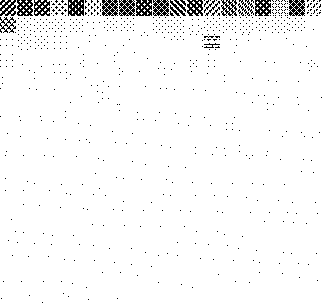
\includegraphics[width=0.9\columnwidth]{fig/einstein_mob_dict.png} %
%
\includegraphics[height=1.55in]{fig/einstein_mob_err_zoom.png}\\[1ex]
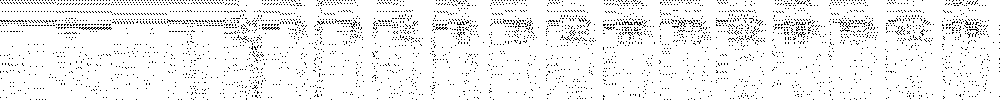
\includegraphics[width=0.9\columnwidth]{fig/einstein_mob_coef_crop.png}
\caption{\label{fig:einstein-mob} Sample model obtained for the Einstein image using MOB. The error in this case is $h(E)=0$, $p=330$, and the dictionary, shown above, follows a similar pattern as that observed in Fig.~\ref{fig:mnist-mob},
 with most of the last atoms being actually just elements from the canonical basis. Below, we show the first $1000$ coefficients corresponding to atoms $1$ to $100$. }
\end{figure}
%
%\begin{figure}
%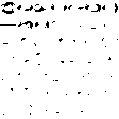
\includegraphics[height=1.7in]{fig/usps_kprox_dict.png}%
%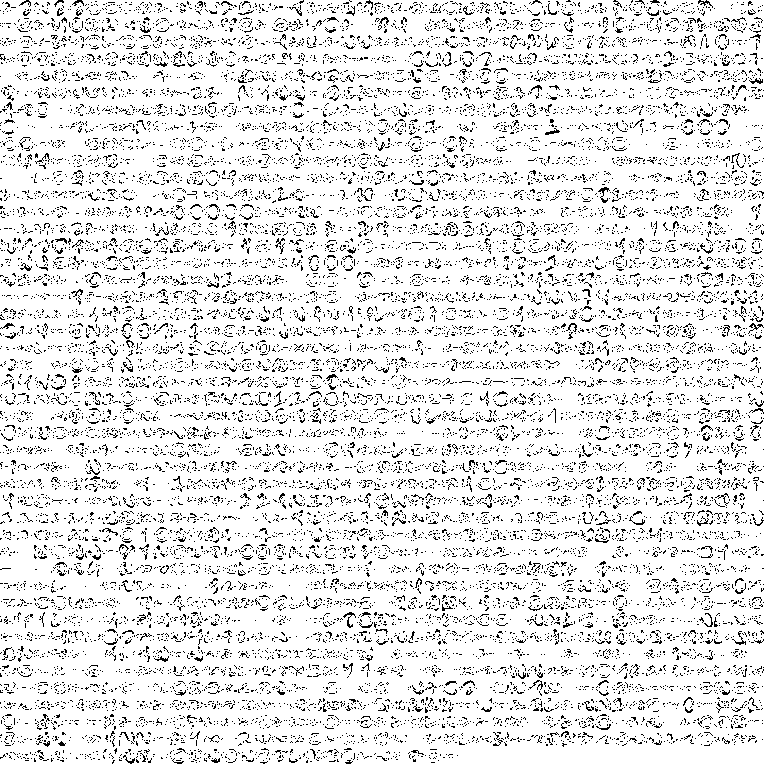
\includegraphics[height=1.7in]{fig/usps_kprox_err.png}\\
%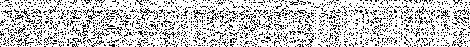
\includegraphics[width=\columnwidth]{fig/usps_kprox_coef_crop.png}
%\caption{\label{fig:usps-kprox} Sample model obtained for the USPS dataset. Left: dictionary. Center: first 100 coefficients. Right: sample residual images. }
%\end{figure}
%
\begin{figure}[tp]
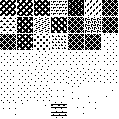
\includegraphics[height=1.55in]{fig/einstein_kprox_dict.png} %
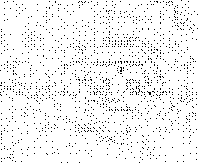
\includegraphics[height=1.55in]{fig/einstein_kprox_err_zoom.png}\\[1ex]
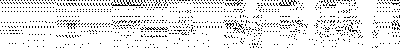
\includegraphics[width=\columnwidth]{fig/einstein_kprox_coef_crop.png}
\caption{\label{fig:einstein-kprox} Model obtained for the Einstein image using K-PROX. In this case the result is quite different from that obtained with MOB. The first atoms are very similar, but the dictinary is much smaller ($p=48$) here lacks most of the finer details represented in that shown in Fig.~\ref{fig:einstein-mob}. Below we show the first $400$ columns of $A$. }
\end{figure}
%
\begin{figure}[tp]
\centering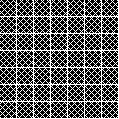
\includegraphics[height=1.0in]{fig/einstein_init_part0.png} % OK
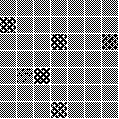
\includegraphics[height=1.0in]{fig/einstein_init_neigh0.png} % OK
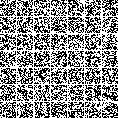
\includegraphics[height=1.0in]{fig/einstein_init_rand0.png}\\[1ex]% OK
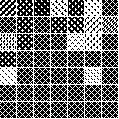
\includegraphics[height=1.0in]{fig/einstein_init_part1.png} % OK
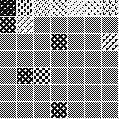
\includegraphics[height=1.0in]{fig/einstein_init_neigh1.png} % OK
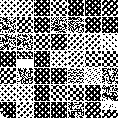
\includegraphics[height=1.0in]{fig/einstein_init_rand1.png}%\\[1ex]% OK
%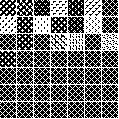
\includegraphics[height=1.1in]{fig/einstein_init_part1_kprox.png} % OK
%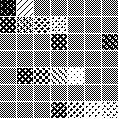
\includegraphics[height=1.1in]{fig/einstein_init_neigh1_kprox.png} % OK
%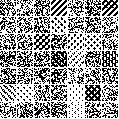
\includegraphics[height=1.1in]{fig/einstein_init_rand1_kprox.png}% OK
\caption{\label{fig:init-einstein} Effect of initialization on Einstein. We show the initial (top), MOB (middle) and K-PROX (bottom) dictionaries obtained by using the pseudo-partition method (left), neighbors (center) and random (right).}
\end{figure}
%
\begin{figure}[tp]
\centering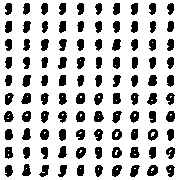
\includegraphics[height=1.0in]{fig/mnist_init_part0.png} % OK
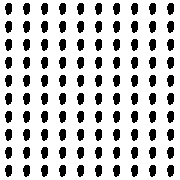
\includegraphics[height=1.0in]{fig/mnist_init_neigh0.png} % OK
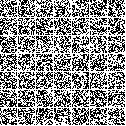
\includegraphics[height=1.0in]{fig/mnist_init_rand0.png}\\[1ex]% OK
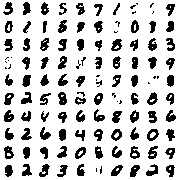
\includegraphics[height=1.0in]{fig/mnist_init_part1.png} % OK
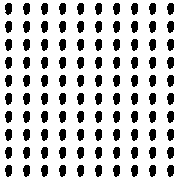
\includegraphics[height=1.0in]{fig/mnist_init_neigh1.png} % OK
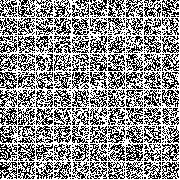
\includegraphics[height=1.0in]{fig/mnist_init_rand1.png}%\\[1ex]% OK
%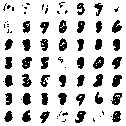
\includegraphics[height=1.1in]{fig/mnist_init_part1_kprox.png} % OK
%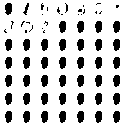
\includegraphics[height=1.1in]{fig/mnist_init_neigh1_kprox.png} % OK
%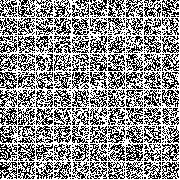
\includegraphics[height=1.1in]{fig/mnist_init_rand1_kprox.png}% OK
\caption{\label{fig:init-mnist} Effect of initialization on MNIST. We show the initial (top), MOB (middle) and K-PROX (bottom) dictionaries obtained by using the pseudo-partition method (left), neighbors (center) and random (right).}
\end{figure}
%

We now show sample models for both datasets, first using the MOB dictionary update, and then using K-PROX. Figure~\ref{fig:mnist-mob} shows the dictionary and a few columns from the coefficients and residial matrices $A$ and $E$; atoms from $D$ and samples from $E$ are represented as mosaics with each sample/atom displayed as a tile. In Figure~\ref{fig:einstein-mob} we show the dictionary, a few columns, and a zoom of the residual image obtained after stitching the patches in their original place. Figures~\ref{fig:mnist-kprox} and ~\ref{fig:einstein-kprox} show the corresponding results using K-PROX.

\subsection{Convergence}
%
\begin{figure*}[tp]
\centering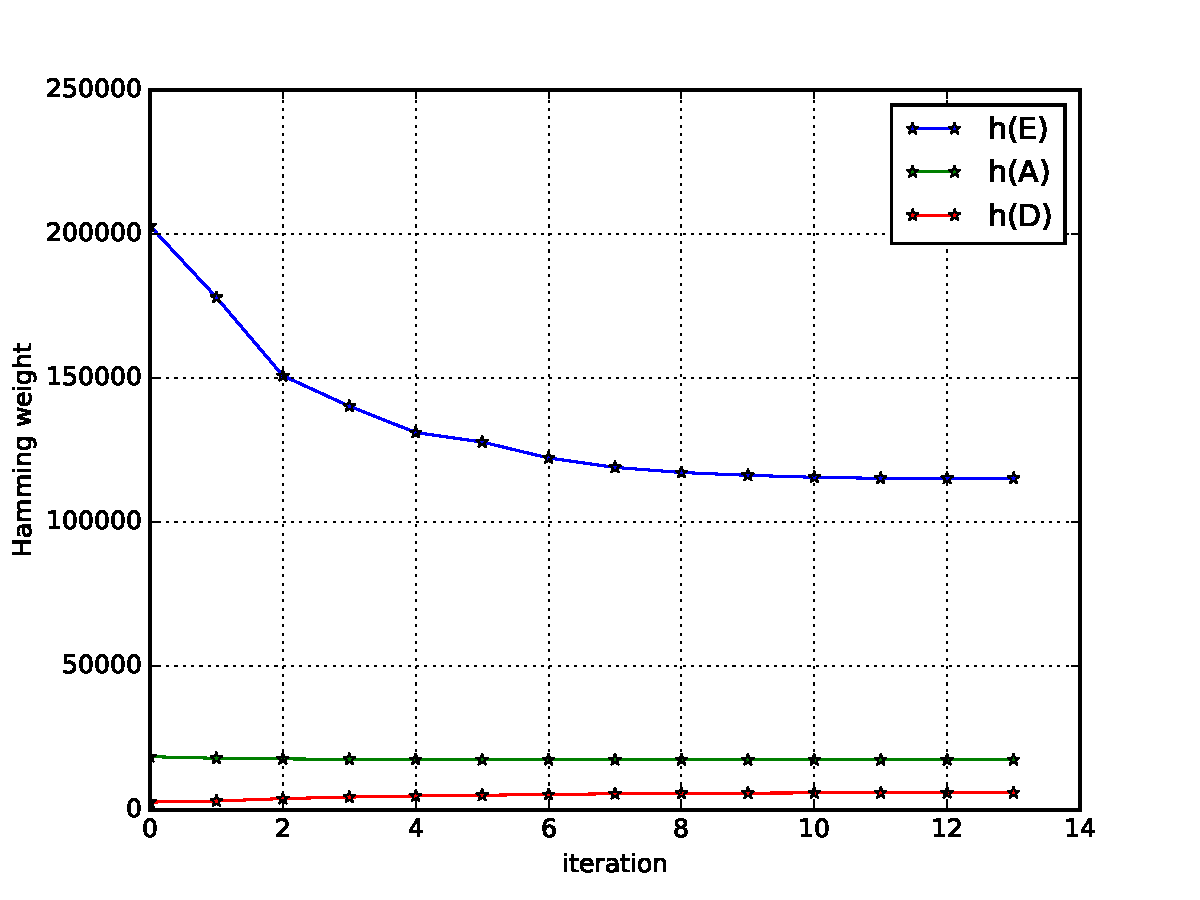
\includegraphics[width=0.45\textwidth]{fig/conv-mob-einstein-h.pdf}%
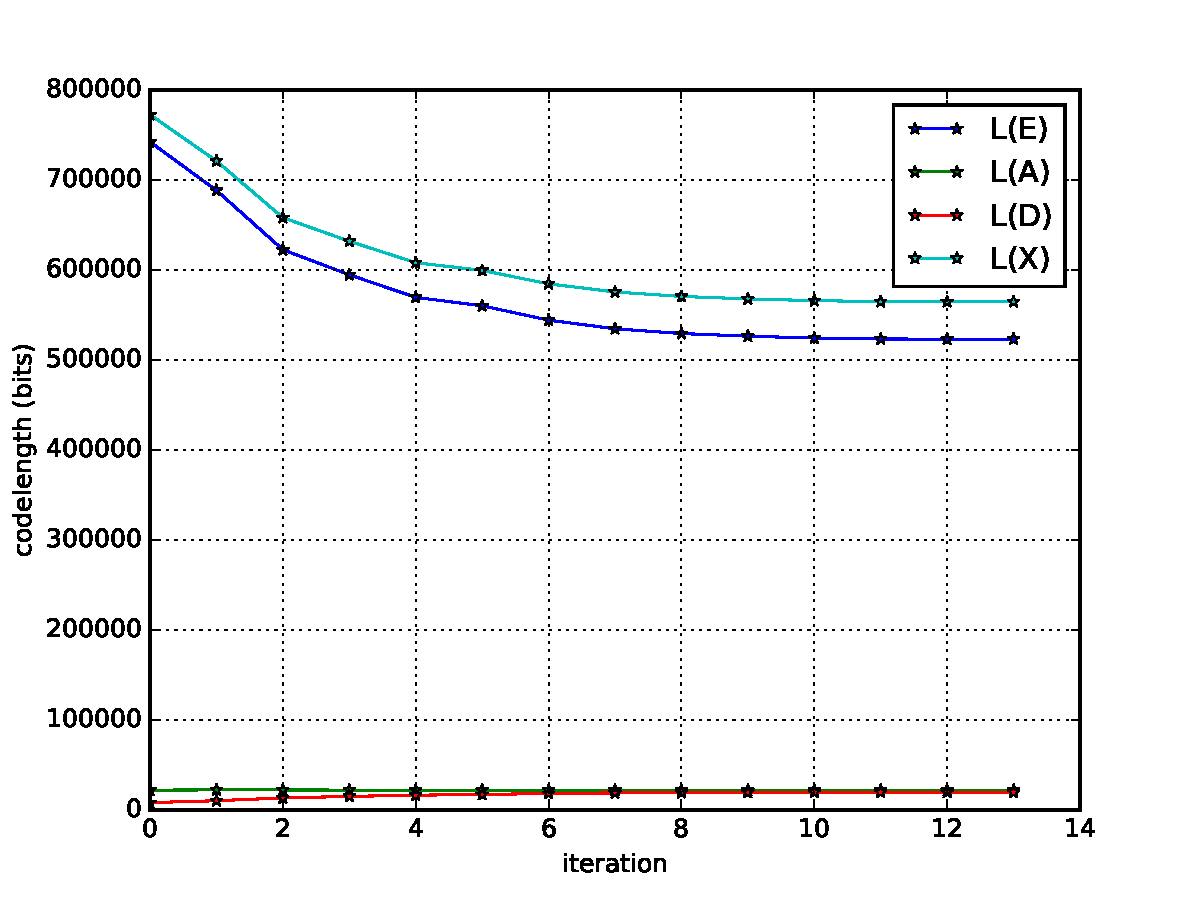
\includegraphics[width=0.45\textwidth]{fig/conv-mob-einstein-L.pdf}\\
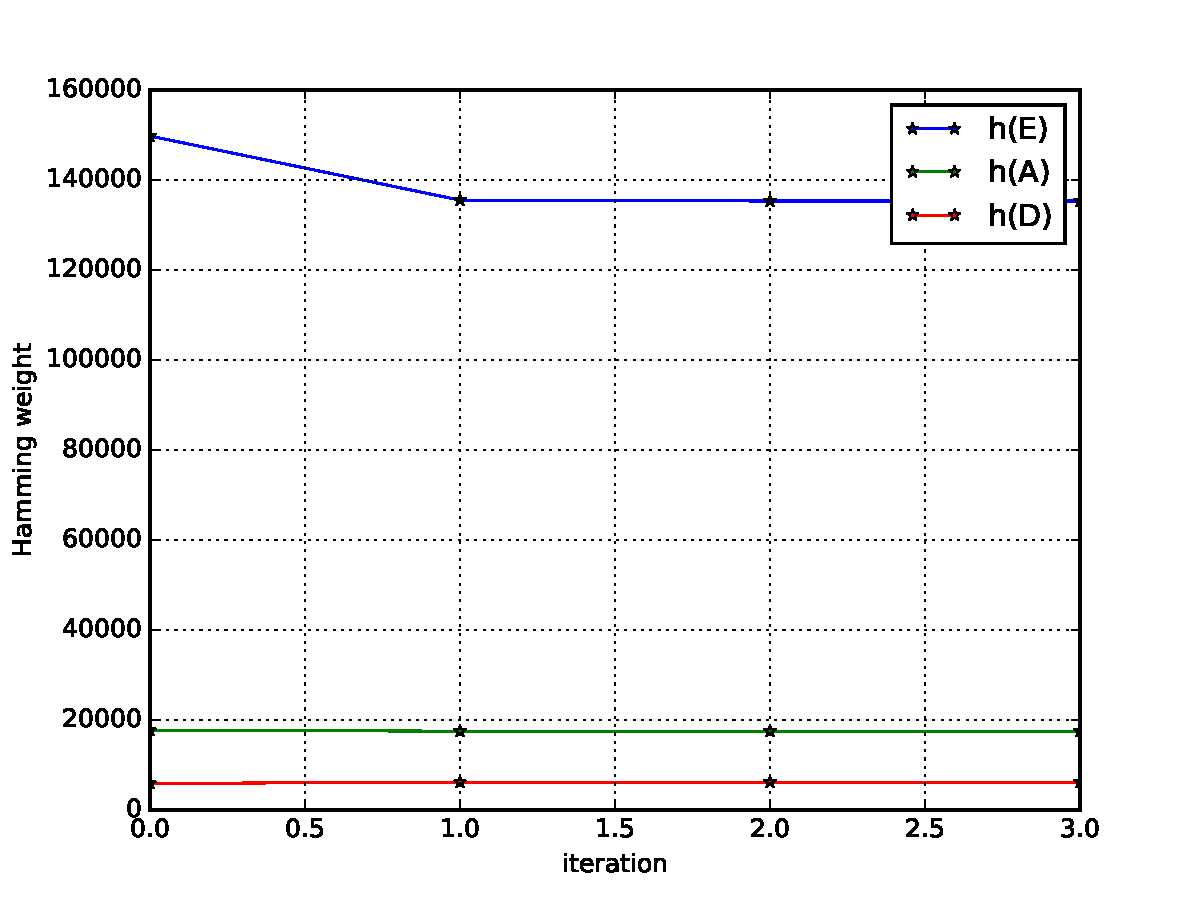
\includegraphics[width=0.45\textwidth]{fig/conv-kprox-einstein-h.pdf}%
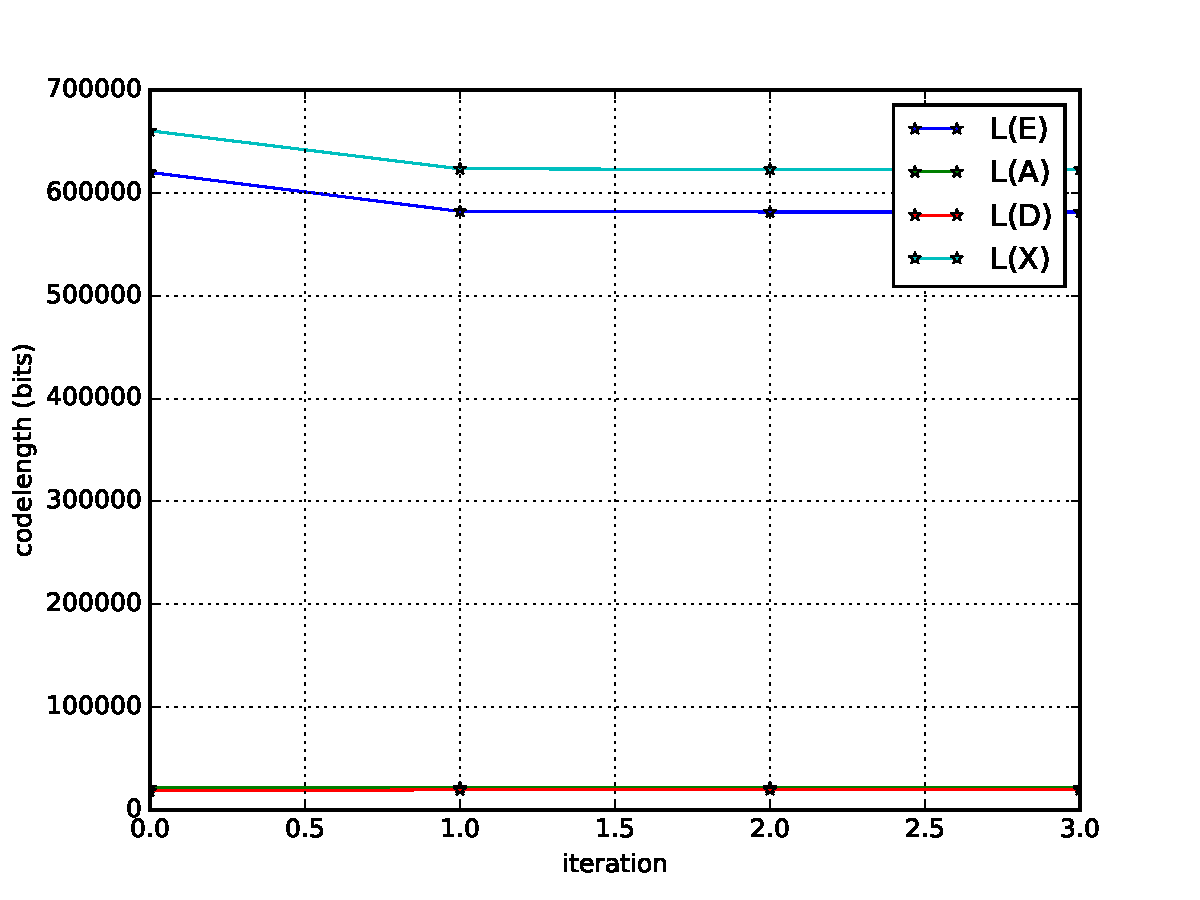
\includegraphics[width=0.45\textwidth]{fig/conv-kprox-einstein-L.pdf}%
\caption{\label{fig:convergence} Convergence results. Above: evolution of Hamming weight (left) and codelength (right) for each component of the matrix factorization using MOB. Below: analogous results using K-PROX. Both methods show a monotonic decrease in Hamming error ($h(E)$) and overall codelength $L(E)$.}
\end{figure*}
Here we analyze the convergence of both methods. Figure~\ref{fig:convergence} shows the results for the two datasets analyzed both in terms of Hamming weight of the solutions and their corresponding codelength. Both MOB and K-PROX are monotonic as expected. We also note that, similarly to K-SVD~\cite{ksvd}, K-PROX achives convergence faster.  Although in these examples it appears to give worse results than MOB, the reader is warned not to generalize such results, as they can be extremely data dependent.

\subsection{Initialization}

Figures~\ref{fig:init-einstein} and~\ref{fig:init-mnist} show initial and final dictionaries of fixed size $p=100$ for MNIST and Einstein, both obtained after initializing the model with the three different methods described in Section~\ref{sec:bdl:init}. As mentioned in Section~\ref{sec:bdl:init}, the neighbor strategy is disastrous for the MNIST case. The same happens with the random initialization.  However, using a random initialization both MOB and K-PROX are able to capture interesting patterns from Einstein after a few iterations. 

\section{Conclusion}
\label{sec:conclusion}

We have presented a novel, efficient Binary Factorization Method based in dictionary learning techniques which, as shown in our preliminary results, is able to capture relevant patterns from the two datasets on which we experimented, both exhibiting quite different characteristics. The methods were analyzed in terms of their convergence and their sensibility to initialization. An online implementation of our proposed methods is currently underway and will be published in a follow up of this publication.

\bibliographystyle{plain}
\bibliography{IEEEabrv,bmf}

\end{document}
